\chapter{Annexos}
\section{Regressions adicionals}
La \cref{tab:regressio forca-angle} i la \cref{fig:forca v rotacio} mostren la regressió lineal realitzada per obtenir la relació entre l'angle de rotació del fil de torsió i la força que exerceix, necessària per a la pràctica \ref{ch:informe 2}.
\begin{table}[htb]
	\centering
	\sffamily
	\small
	\caption{Força del fil de torsió en funció de l'angle}
	\label{tab:regressio forca-angle}
	\begin{tabular}{SS}
		\toprule
		{Massa (\si{mg})} & {Rotació (\si{\degree}) (\( {} \pm \SI{1}{\degree} \))} \\
		\midrule
		5 & 13 \\
		10 & 27 \\
		15 & 44 \\
		20 & 63 \\
		25 & 70 \\
		\bottomrule
	\end{tabular}
\end{table}

\begin{figure}[htb]
	\centering
	% GNUPLOT: LaTeX picture with Postscript
\begingroup
\sffamily \small
  \makeatletter
  \providecommand\color[2][]{%
    \GenericError{(gnuplot) \space\space\space\@spaces}{%
      Package color not loaded in conjunction with
      terminal option `colourtext'%
    }{See the gnuplot documentation for explanation.%
    }{Either use 'blacktext' in gnuplot or load the package
      color.sty in LaTeX.}%
    \renewcommand\color[2][]{}%
  }%
  \providecommand\includegraphics[2][]{%
    \GenericError{(gnuplot) \space\space\space\@spaces}{%
      Package graphicx or graphics not loaded%
    }{See the gnuplot documentation for explanation.%
    }{The gnuplot epslatex terminal needs graphicx.sty or graphics.sty.}%
    \renewcommand\includegraphics[2][]{}%
  }%
  \providecommand\rotatebox[2]{#2}%
  \@ifundefined{ifGPcolor}{%
    \newif\ifGPcolor
    \GPcolortrue
  }{}%
  \@ifundefined{ifGPblacktext}{%
    \newif\ifGPblacktext
    \GPblacktextfalse
  }{}%
  % define a \g@addto@macro without @ in the name:
  \let\gplgaddtomacro\g@addto@macro
  % define empty templates for all commands taking text:
  \gdef\gplbacktext{}%
  \gdef\gplfronttext{}%
  \makeatother
  \ifGPblacktext
    % no textcolor at all
    \def\colorrgb#1{}%
    \def\colorgray#1{}%
  \else
    % gray or color?
    \ifGPcolor
      \def\colorrgb#1{\color[rgb]{#1}}%
      \def\colorgray#1{\color[gray]{#1}}%
      \expandafter\def\csname LTw\endcsname{\color{white}}%
      \expandafter\def\csname LTb\endcsname{\color{black}}%
      \expandafter\def\csname LTa\endcsname{\color{black}}%
      \expandafter\def\csname LT0\endcsname{\color[rgb]{1,0,0}}%
      \expandafter\def\csname LT1\endcsname{\color[rgb]{0,1,0}}%
      \expandafter\def\csname LT2\endcsname{\color[rgb]{0,0,1}}%
      \expandafter\def\csname LT3\endcsname{\color[rgb]{1,0,1}}%
      \expandafter\def\csname LT4\endcsname{\color[rgb]{0,1,1}}%
      \expandafter\def\csname LT5\endcsname{\color[rgb]{1,1,0}}%
      \expandafter\def\csname LT6\endcsname{\color[rgb]{0,0,0}}%
      \expandafter\def\csname LT7\endcsname{\color[rgb]{1,0.3,0}}%
      \expandafter\def\csname LT8\endcsname{\color[rgb]{0.5,0.5,0.5}}%
    \else
      % gray
      \def\colorrgb#1{\color{black}}%
      \def\colorgray#1{\color[gray]{#1}}%
      \expandafter\def\csname LTw\endcsname{\color{white}}%
      \expandafter\def\csname LTb\endcsname{\color{black}}%
      \expandafter\def\csname LTa\endcsname{\color{black}}%
      \expandafter\def\csname LT0\endcsname{\color{black}}%
      \expandafter\def\csname LT1\endcsname{\color{black}}%
      \expandafter\def\csname LT2\endcsname{\color{black}}%
      \expandafter\def\csname LT3\endcsname{\color{black}}%
      \expandafter\def\csname LT4\endcsname{\color{black}}%
      \expandafter\def\csname LT5\endcsname{\color{black}}%
      \expandafter\def\csname LT6\endcsname{\color{black}}%
      \expandafter\def\csname LT7\endcsname{\color{black}}%
      \expandafter\def\csname LT8\endcsname{\color{black}}%
    \fi
  \fi
    \setlength{\unitlength}{0.0500bp}%
    \ifx\gptboxheight\undefined%
      \newlength{\gptboxheight}%
      \newlength{\gptboxwidth}%
      \newsavebox{\gptboxtext}%
    \fi%
    \setlength{\fboxrule}{0.5pt}%
    \setlength{\fboxsep}{1pt}%
\begin{picture}(5668.00,3400.00)%
    \gplgaddtomacro\gplbacktext{%
      \csname LTb\endcsname%%
      \put(1078,704){\makebox(0,0)[r]{\strut{}\num{0}}}%
      \put(1078,1117){\makebox(0,0)[r]{\strut{}\num{0.05}}}%
      \put(1078,1529){\makebox(0,0)[r]{\strut{}\num{0.1}}}%
      \put(1078,1942){\makebox(0,0)[r]{\strut{}\num{0.15}}}%
      \put(1078,2354){\makebox(0,0)[r]{\strut{}\num{0.2}}}%
      \put(1078,2767){\makebox(0,0)[r]{\strut{}\num{0.25}}}%
      \put(1078,3179){\makebox(0,0)[r]{\strut{}\num{0.3}}}%
      \put(1210,484){\makebox(0,0){\strut{}\num{10}}}%
      \put(1790,484){\makebox(0,0){\strut{}\num{20}}}%
      \put(2370,484){\makebox(0,0){\strut{}\num{30}}}%
      \put(2950,484){\makebox(0,0){\strut{}\num{40}}}%
      \put(3531,484){\makebox(0,0){\strut{}\num{50}}}%
      \put(4111,484){\makebox(0,0){\strut{}\num{60}}}%
      \put(4691,484){\makebox(0,0){\strut{}\num{70}}}%
      \put(5271,484){\makebox(0,0){\strut{}\num{80}}}%
    }%
    \gplgaddtomacro\gplfronttext{%
      \csname LTb\endcsname%%
      \put(198,1941){\rotatebox{-270}{\makebox(0,0){\strut{}$\mathsf{F \ (\si{mN})}$}}}%
      \put(3240,154){\makebox(0,0){\strut{}$\mathsf{\theta \ (\si{\degree})}$}}%
    }%
    \gplbacktext
    \put(0,0){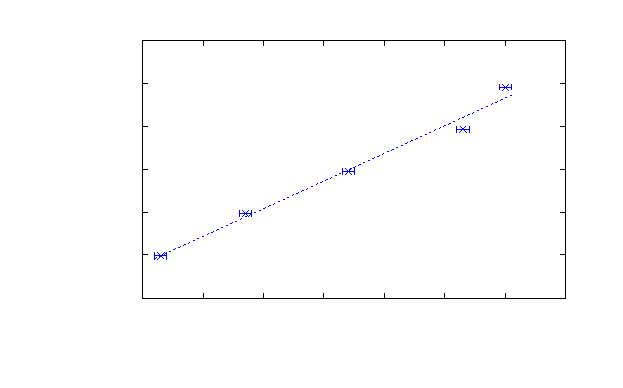
\includegraphics{forca-rotacio}}%
    \gplfronttext
  \end{picture}%
\endgroup

	\caption{Força en funció de la rotació del dial}
	\label{fig:forca v rotacio}
\end{figure}


\newpage
\section{Taules amb dades adicionals}
\begin{table}[p] 
	\centering \footnotesize \sffamily
	\caption{Mesures experimentals de la resistència a diferents temperatures. El voltatge subministrat és de \data{3.1}{0.2}{V}}
	\label{tab:temp i resistencia}
	\begin{tabular}{SSS}
		\toprule
		{Temperatura (\data{}{1}{\celsius}) } & {Longitud \( x \) (\data{}{0.001}{m})} & {Resistència (\si{\ohm})} \\
		\midrule
		265 & 0.664 & 198 \pm 9 \\
		260 & 0.668 & 201 \pm 9 \\
		255 & 0.665 & 199 \pm 9 \\
		250 & 0.664 & 198 \pm 9 \\
		245 & 0.663 & 197 \pm 9 \\
		240 & 0.661 & 195 \pm 9 \\
		235 & 0.659 & 193 \pm 9 \\
		230 & 0.657 & 192 \pm 9 \\
		225 & 0.655 & 190 \pm 9 \\
		220 & 0.654 & 189 \pm 9 \\
		210 & 0.646 & 182 \pm 8 \\
		200 & 0.643 & 180 \pm 8 \\
		190 & 0.637 & 175 \pm 8 \\
		180 & 0.630 & 170 \pm 8 \\
		170 & 0.627 & 168 \pm 7 \\
		160 & 0.622 & 165 \pm 7 \\
		155 & 0.620 & 163 \pm 7 \\
		150 & 0.616 & 160 \pm 7 \\
		145 & 0.613 & 158 \pm 7 \\
		140 & 0.610 & 156 \pm 7 \\
		135 & 0.608 & 155 \pm 7 \\
		130 & 0.605 & 153 \pm 7 \\
		125 & 0.603 & 152 \pm 7 \\
		120 & 0.600 & 150 \pm 6 \\
		115 & 0.597 & 148 \pm 6 \\
		110 & 0.593 & 146 \pm 6 \\
		105 & 0.585 & 141 \pm 6 \\
		23 & 0.520 & 108 \pm 5 \\
		-20 & 0.485 & 94 \pm 4{}\\
		-25 & 0.484 & 94 \pm 4 \\
		-30 & 0.481 & 93 \pm 4 \\
		-35 & 0.478 & 92 \pm 4 \\
		-40 & 0.474 & 90 \pm 4 \\
		-45 & 0.470 & 88 \pm 4 \\
		-49 & 0.468 & 88 \pm 4 \\
		-55 & 0.464 & 87 \pm 4 \\
		-60 & 0.459 & 85 \pm 4 \\
		-65 & 0.457 & 84 \pm 4 \\
		-70 & 0.452 & 82 \pm 3 \\
		-75 & 0.447 & 81 \pm 3 \\
		-80 & 0.445 & 80 \pm 3 \\
		-85 & 0.441 & 79 \pm 3 \\
		-90 & 0.436 & 77 \pm 3 \\
		-95 & 0.431 & 76 \pm 3 \\
		-100 & 0.424 & 74 \pm 3 \\
		-105 & 0.417 & 72 \pm 3 \\
		-110 & 0.409 & 69 \pm 3 \\
		-115 & 0.398 & 66 \pm 3 \\
		-150 & 0.365 & 57 \pm 3 \\
		\bottomrule
	\end{tabular}
\end{table}

A la \cref{tab:forca v intensitat (detall)} hi ha les intensitats mesurades per a cada massa, referent a la pràctica \ref{ch:informe 2}.
\begin{table}[htb]
	\centering
	\sffamily \small
	\caption{Mesures de la intensitat necessària per contrarrestar la força gravitatòria de cada massa}
	\label{tab:forca v intensitat (detall)}
	\begin{tabular}{SSSSSSS}
		\toprule	
		{Massa (\si{mg})} & \multicolumn{6}{c}{Intensitat (\data{}{0.01}{A})} \\
		\midrule 
		5 & 2.62 & 2.55 & 2.65 & 2.62 & 2.60 & 2.57 \\
		10 & 3.70 & 3.40 & 3.58 & 3.64 & 3.71 & 3.68 \\
		15 & 4.47 & 4.46 & 4.63 & 4.42 & 4.50 & 4.48 \\
		20 & 5.10 & 5.29 & 5.33 & 5.07 & 5.10 & 5.11 \\
		25 & 6.05 & 5.99 & 5.94 & 5.40 & 5.21 & 5.63 \\
		\bottomrule
	\end{tabular}
\end{table}

A la \cref{tab:temp i resistencia} hi ha la resistència mesurada per a cada temperatura, referent a la pràctica \ref{ch:informe 5}.

\newpage
\section{Codis per a les simulacions}\label{sec:codis}
A continuació es presenten els codis emprats per a les simulacions de la pràctica \ref{ch:informe 1}
\lstinputlisting[language=C, caption=Codi per a calcular el potencial degut a un condensador fent servir l'algoritme de Jacobi, label={lst:condensador}]{informe-1/figs/codis/simulacio-condensador.c}

\lstinputlisting[language=C, caption=Codi per a calcular el potencial degut a dos fils fent servir l'algoritme de Jacobi, label={lst:fils}]{informe-1/figs/codis/simulacio-fils.c}

\lstinputlisting[language=C, caption=Codi per a calcular el potencial degut a la configuraci\'o lliure fent servir l'algoritme de Jacobi, label={lst:lliure}]{informe-1/figs/codis/simulacio-lliure.c}
